This section will outline the approaches taken to develop and compare a suite of
classifier models as well as the gathering and preparation of a custom coffee
bean defect dataset.

\section{Sample gathering and dataset development}
\label{sec:sample-gathering-and-dataset-development} At the early stages of the
project, it became clear that public coffee bean image datasets will not be suitable
for the aims of this project as they often lack in variety of defects as well as
suffer from a lack of labelling in that regard.
Therefore, a custom dataset,
reflecting the variety of existing defects and coffee varieties was necessary to
ensure that any developed model can cope with the diversity of coffee available
on the market.

The gathered dataset consisted of roughly two kilograms of roasted coffee, gathered
from two small-scale coffee roasters: Harmony Roasters based in York and Vibe
With coffee based in Nottingham.
Both roasters are in the specialty coffee market
and switch their offerings frequently, allowing them to work with a variety of
coffee suppliers and species.
Both roasters mentioned performing manual quality control
after every roast session and expressed interest in the automation of this process,
echoing the research aims of the project.

Over a period of 6 weeks between november and february 2023, both roasters were asked
to keep track of any defective beans they come across and separate the defects by
the variety the coffee belonged to.
This ensured that the roasters were not
asked to spend too much of their time and could still perform their usual duties
with as little distraction as possible.
Neither roaster asked for compensation for
their work, however, samples of non-defective beans were purchased for their usual
retail price, ensuring that the research process would not take any advantage of
their time and effort.

Upon gathering the beans, the defective beans were inspected once again with each
defect separated into its own section.
The separation was done after a
consultation with the coffee roasters, who provided a verbal description of each
defect's visual characteristics.
The non-defective beans were also double-checked
for any defects in order to ensure the least amount of incorrectly labelled
samples.

To digitize the dataset, beans of each group were arranged in $5 \times 5$ grids
(where possible) and photographed using the main lens of the Pixel 7 pro smartphone.
All images were taken on a bright white background, with care taken to not include any dust or debris in the image.
Overhead lights along with a smaller tabletop light were used to make sure lighting levels stayed consistent between pictures.
Images of each defect were stored locally on the smartphone with a backup made
in google images and GitHub.

Overall, the dataset contained 2786 images, each annotated with the bean variety,
the processing method used and the defect (or lack thereof) present in the bean.
It should be noted that despite the initial aims, the distribution of defects in
the final dataset was imbalanced, with certain defects occuring much less
frequently than others.
To attempt to combat this, in cases where a bean
exhibited several defects at once, it was labelled as the rarer defect.
For
example, if the bean was both a ''quaker`` (underdeveloped) and had insect damage,
it was labelled as having insect damage only.
While not a perfect solution, this
ensured a satisfactory number of images per class.
A further description of the dataset
is provided below.

\subsection{Dataset description and statistics}
\label{subsec:dataset-description-and-statistics}
\begin{figure}[h]
{\textwidth}
	\begin{subfigure}
	{0.2\textwidth}
		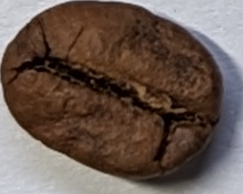
\includegraphics[height=0.8\linewidth, keepaspectratio]{
			./figures/methodology/quaker-bean
		}
		\subcaption{''Quaker``} \label{fig:quakerBeanSingle}
	\end{subfigure}
	\begin{subfigure}
	{0.2\textwidth}
		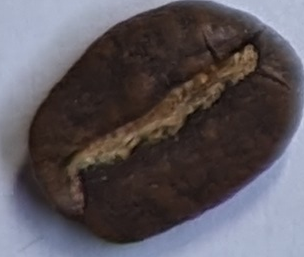
\includegraphics[height=0.8\linewidth, keepaspectratio]{
			./figures/methodology/normal-bean
		}
		\subcaption{Normal} \label{fig:normalBeanSingle}
	\end{subfigure}
	\begin{subfigure}
	{0.2\textwidth}
		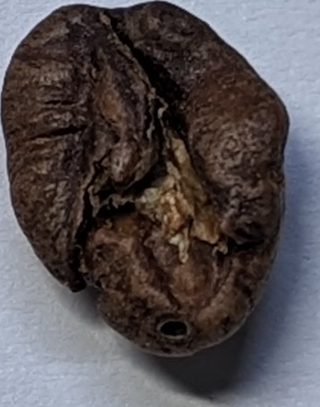
\includegraphics[height=0.8\linewidth, keepaspectratio]{
			./figures/methodology/insect-damaged-bean
		}
		\subcaption{Insect \\ damage} \label{fig:insectBeanSingle}
	\end{subfigure}
	\begin{subfigure}
	{0.2\textwidth}
		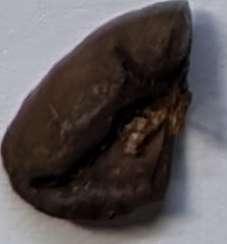
\includegraphics[height=0.8\linewidth, keepaspectratio]{
			./figures/methodology/bean-fragment
		}
		\subcaption{Bean \\ fragment} \label{fig:fragBeanSingle}
	\end{subfigure}
	\begin{subfigure}
	{0.25\textwidth}
		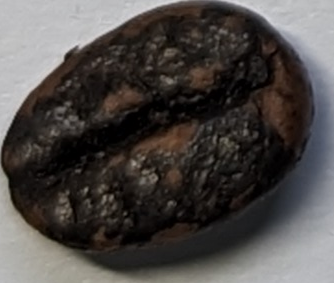
\includegraphics[height=0.8\linewidth, keepaspectratio]{
			./figures/methodology/burnt-bean
		}
		\subcaption{Burnt} \label{fig:burntBeanSingle}
	\end{subfigure}
	\begin{subfigure}
	{0.25\textwidth}
		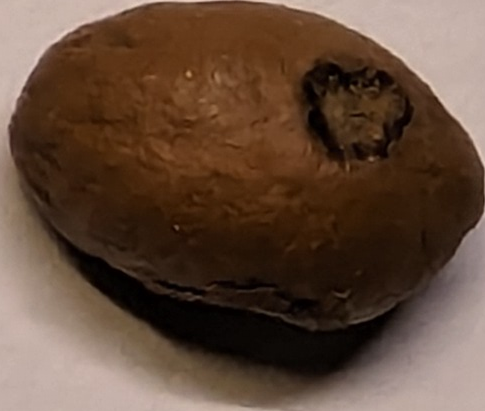
\includegraphics[height=0.8\linewidth, keepaspectratio]{
			./figures/methodology/mold-damaged-bean
		}
		\subcaption{Mould damage} \label{fig:moldBeanSingle}
	\end{subfigure}
	\begin{subfigure}
	{0.25\textwidth}
		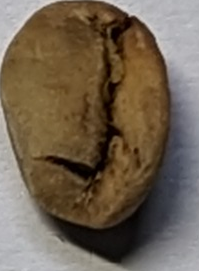
\includegraphics[height=0.8\linewidth, keepaspectratio]{
			./figures/methodology/under-bean
		}
		\subcaption{Underroasted} \label{fig:underBeanSingle}
	\end{subfigure}
	\caption{Examples of bean defects}
	\label{fig:beanDefects}
\end{figure}

Keeping in line with the project
aims, this section will mainly focus on the defects identified in the beans
contained in the dataset.
Overall, the beans exhibited five various defects, whose
counts and short descriptions are presented in table~\ref{tab:beanDefectCounts}.
Figure~\ref{fig:beanDefects} provides a brief look at the various defects, with more
examples shown in the appendix % TODO add appendix with more images

\begin{table}[h]
	\centering
	\begin{tabular}{|p{0.25\linewidth}|p{0.6\linewidth}|p{0.15\linewidth}|}
		\toprule \textbf{Defect name} & \textbf{Visual features}                                                                                                                                             & \textbf{Count} \\
		\midrule Normal bean          & Even colour, brown to dark-brown hue, no surface damage or blemishes and a round shape with no deformities                                                           & 1311           \\
		Quaker                        & Light brown to brown hue (due to less caramelisation of sugar), scorch marks, brown spots on surface.
		Occasionally, a shrivelled, uneven look of the outside surface & 978            \\
		Bean fragment                 & Significantly deformed or chipped exterior, smaller bean pieces                                                                                                      & 296            \\
		Underroasted                  & Very light brown exterior, dark green or yellow in extremely underroasted beans                                                                                      & 104            \\
		Burnt                         & Dark brown to black exterior, significant scorching or an oily, shiny surface                                                                                        & 50             \\
		Insect/mould damage           & Small, round holes or larger ''craters`` on the surface                                                                                                              & 47             \\
		\bottomrule
	\end{tabular}
	\caption{Bean defect counts}
	\label{tab:beanDefectCounts}
\end{table}

The beans in the dataset belonged to a total of nine varieties and have been processed using six different methods.
The number of beans belonging to each processing method and variety method is shown
on figures~\ref{fig:beanProcessingCounts} and~\ref{fig:beanVarietyCounts} respectively.
\begin{figure}[h]
	\centering
		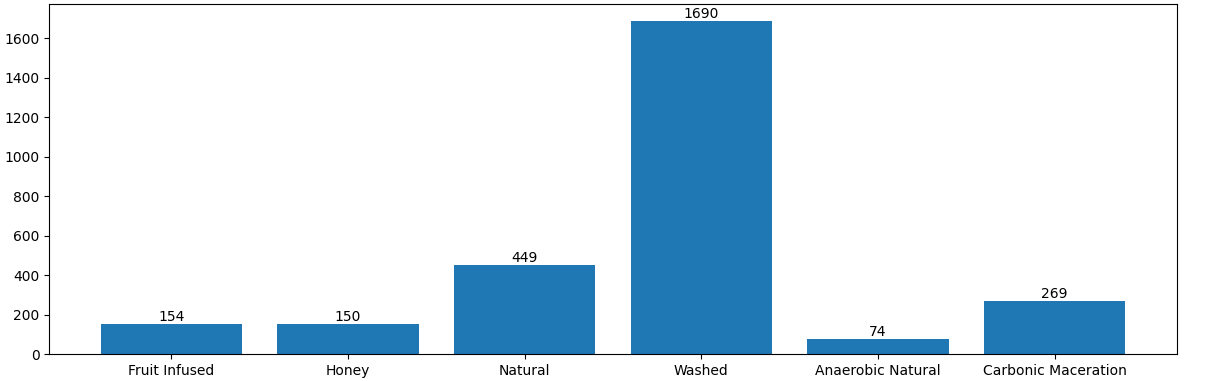
\includegraphics[width=\linewidth, height=2.5cm]{
			./figures/methodology/processing-counts
		}
	\caption{Bean processing method counts}
	\label{fig:beanProcessingCounts}

	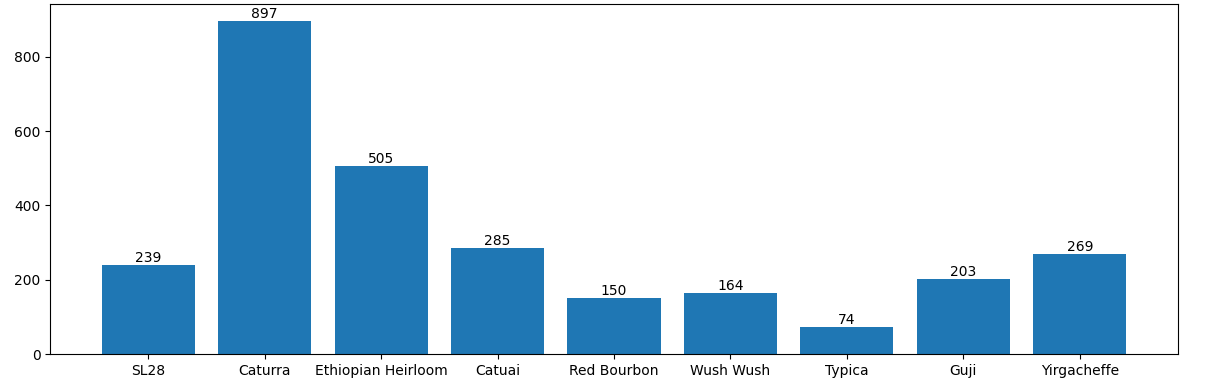
\includegraphics[width=\linewidth, height=2.5cm]{
			./figures/methodology/variety-counts
		}
	\caption{Bean variety counts}
	\label{fig:beanVarietyCounts}
\end{figure}

It should be noted that the original intent was for the insect and mould damage to be distinct classes,
however, these defects are quite rare, especially with the higher-grade green coffee the local roasters worked with.
Because of this lack of available data, it was decided to merge the classes: not only do the visual features of the two
defects resemble each other, but the effects they have on the final product are also similar.
While future work could seek an improved dataset and a higher granularity of classes, the merging of the two classes here
is unlikely to reduce the practical usefulness of the classifier in a roaster's daily tasks.
\subsection{Data pre-processing}
\label{subsec:data-pre-processing}
As described in the above section, the beans were arranged in grids when their pictures were taken.
To train the classifier however, each bean had to be contained in its own image, requiring the use of a software solution
to automatically separate each bean.
The solution was implemented in Python and depended heavily on the OpenCV library~\cite{opencvLibrary}, which provides
tools for working with and processing images.

Separating the grid images involved several steps.
First, the image was loaded and converted to grayscale using a built-in OpenCV function.
Then, a threshold was applied to the resulting images to provide a binary separation between the beans and the background.
An important step was inverting the thresholded images so that the background was represented by black pixels
and the beans by white ones - this was required for the contour finding step that followed.

Once the binary images were produced, the \verb |findContours| function was used to identify the contours and
bounding rectangles of each individual bean.
At this stage, additional checks were conducted to ensure that no dust or foreign objects were captured by the algorithm:
bounding rectangles whose areas were uncharacteristically small or large or whose aspect ratio was too imbalanced were rejected.
The expected dimensions were gathered by running the algorithm once and inspecting the produced images: the images tended
to be around 200--400 pixels wide/tall, with an aspect ratio not exceeding 1:3.
Finally, the batch images were separated into sections matching the positions and dimensions of each bounding rectangle.
The resulting images were named reflecting the bean's variety, origin, processing method and defect class and sorted into folders
named in the same pattern.
A CSV file reflecting the class annotations has also been generated and stored in the image directory.
Each row in the CSV file corresponded to a single bean, with the columns containing the image name and the
aforementioned class information.

A visualisation of the data processing pipeline is shown on figure~\ref{fig:imgProcessing}.
\pagebreak
\begin{figure}[h]
	\centering
\begin{tikzpicture}
	\node (raw)
		{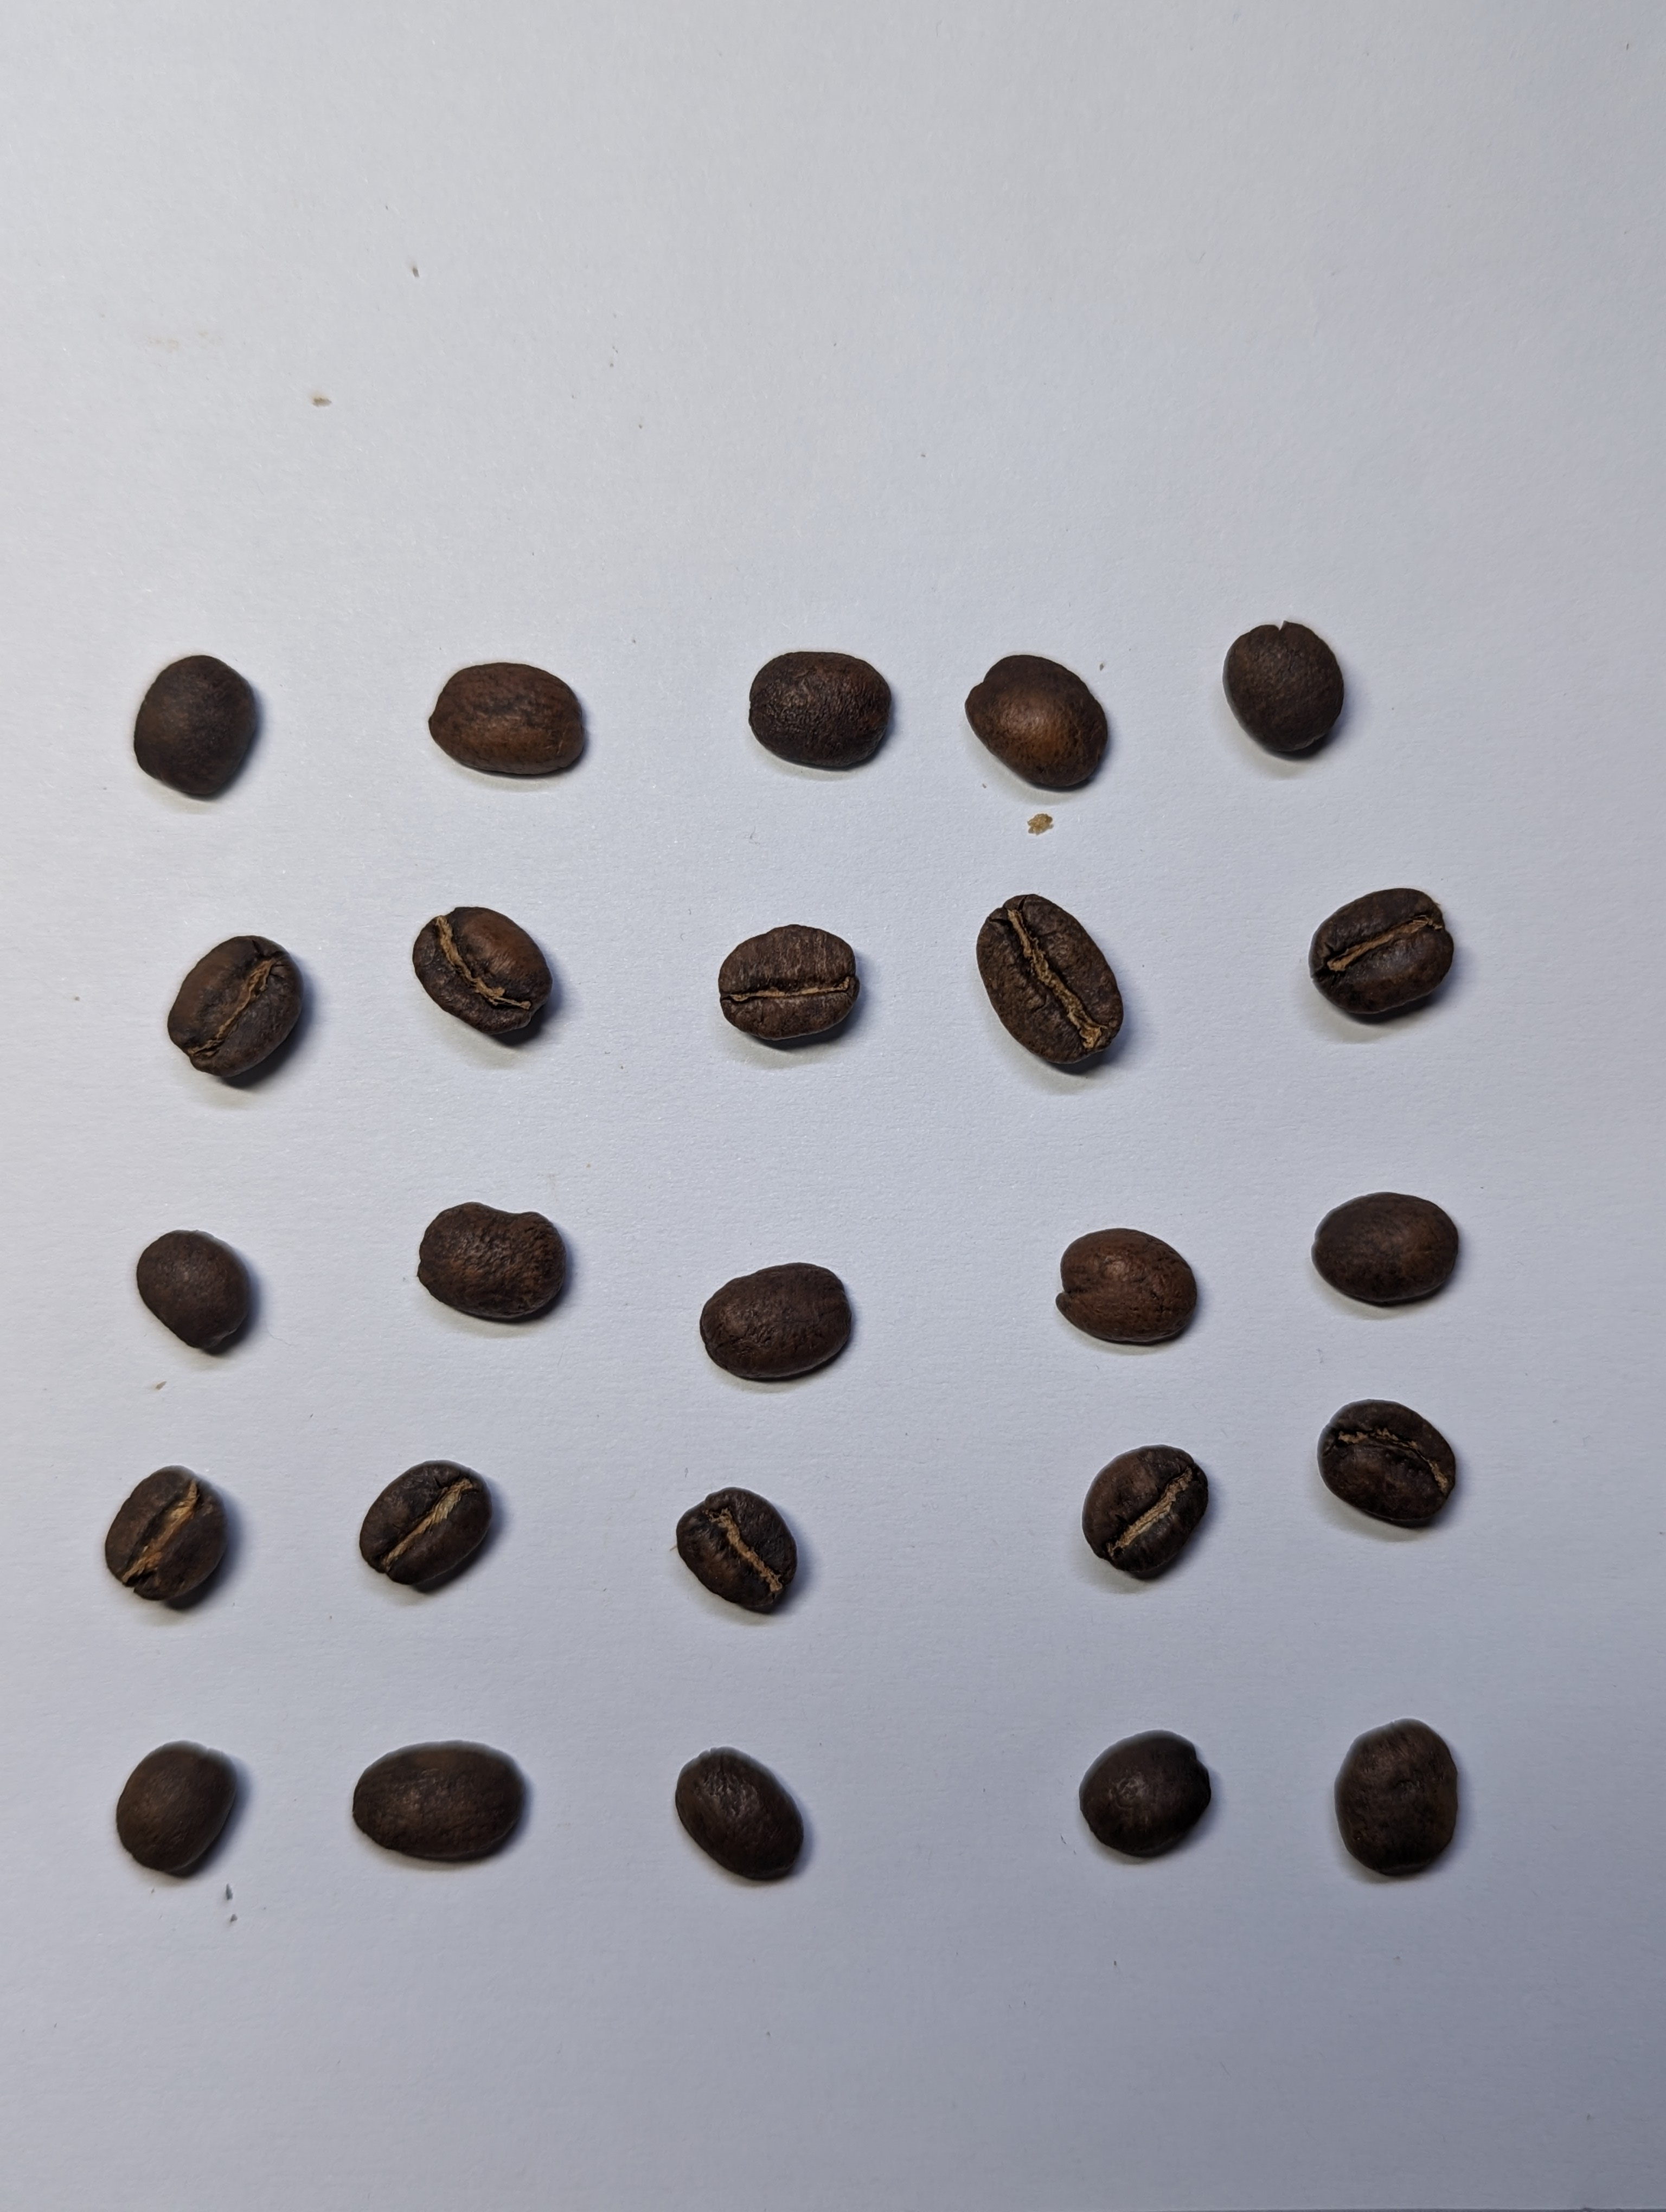
\includegraphics[height=4cm, keepaspectratio]{methodology/bean-batch-raw}};
	\node[right=of raw](gray)
		{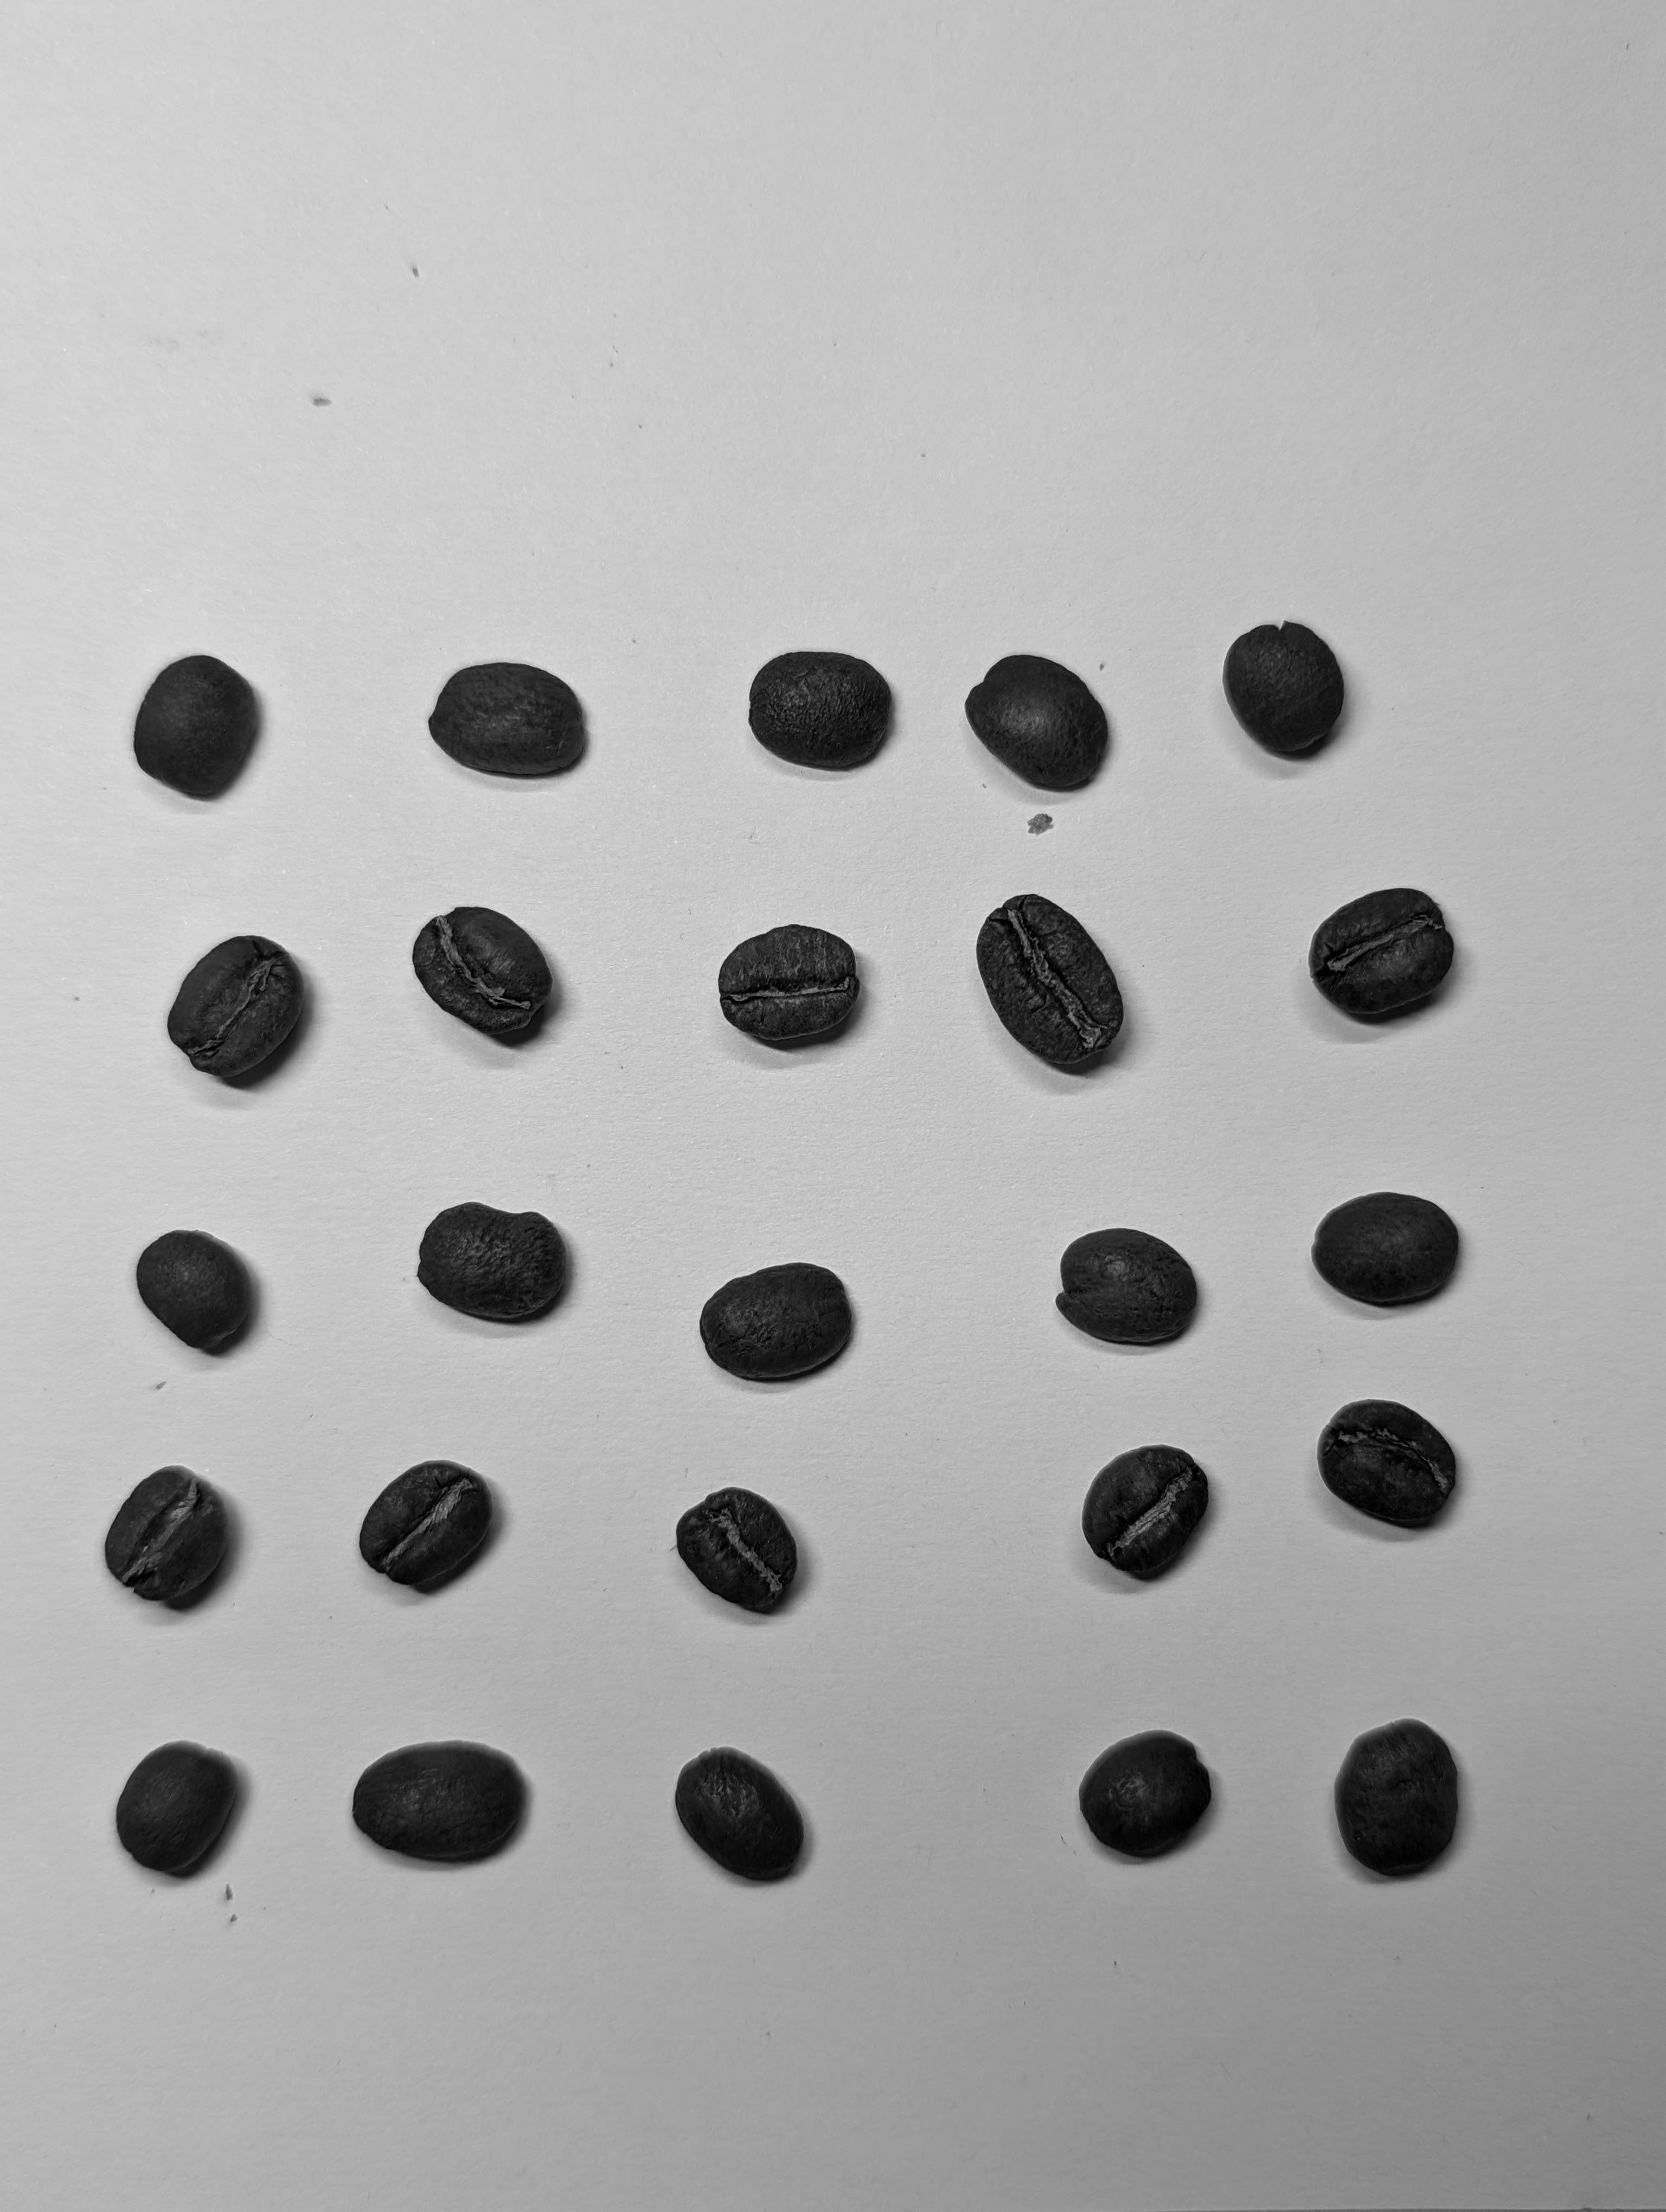
\includegraphics[height=4cm, keepaspectratio]{methodology/bean-batch-gray}};
	\node[left=of thresh, below=of raw] (contours)
		{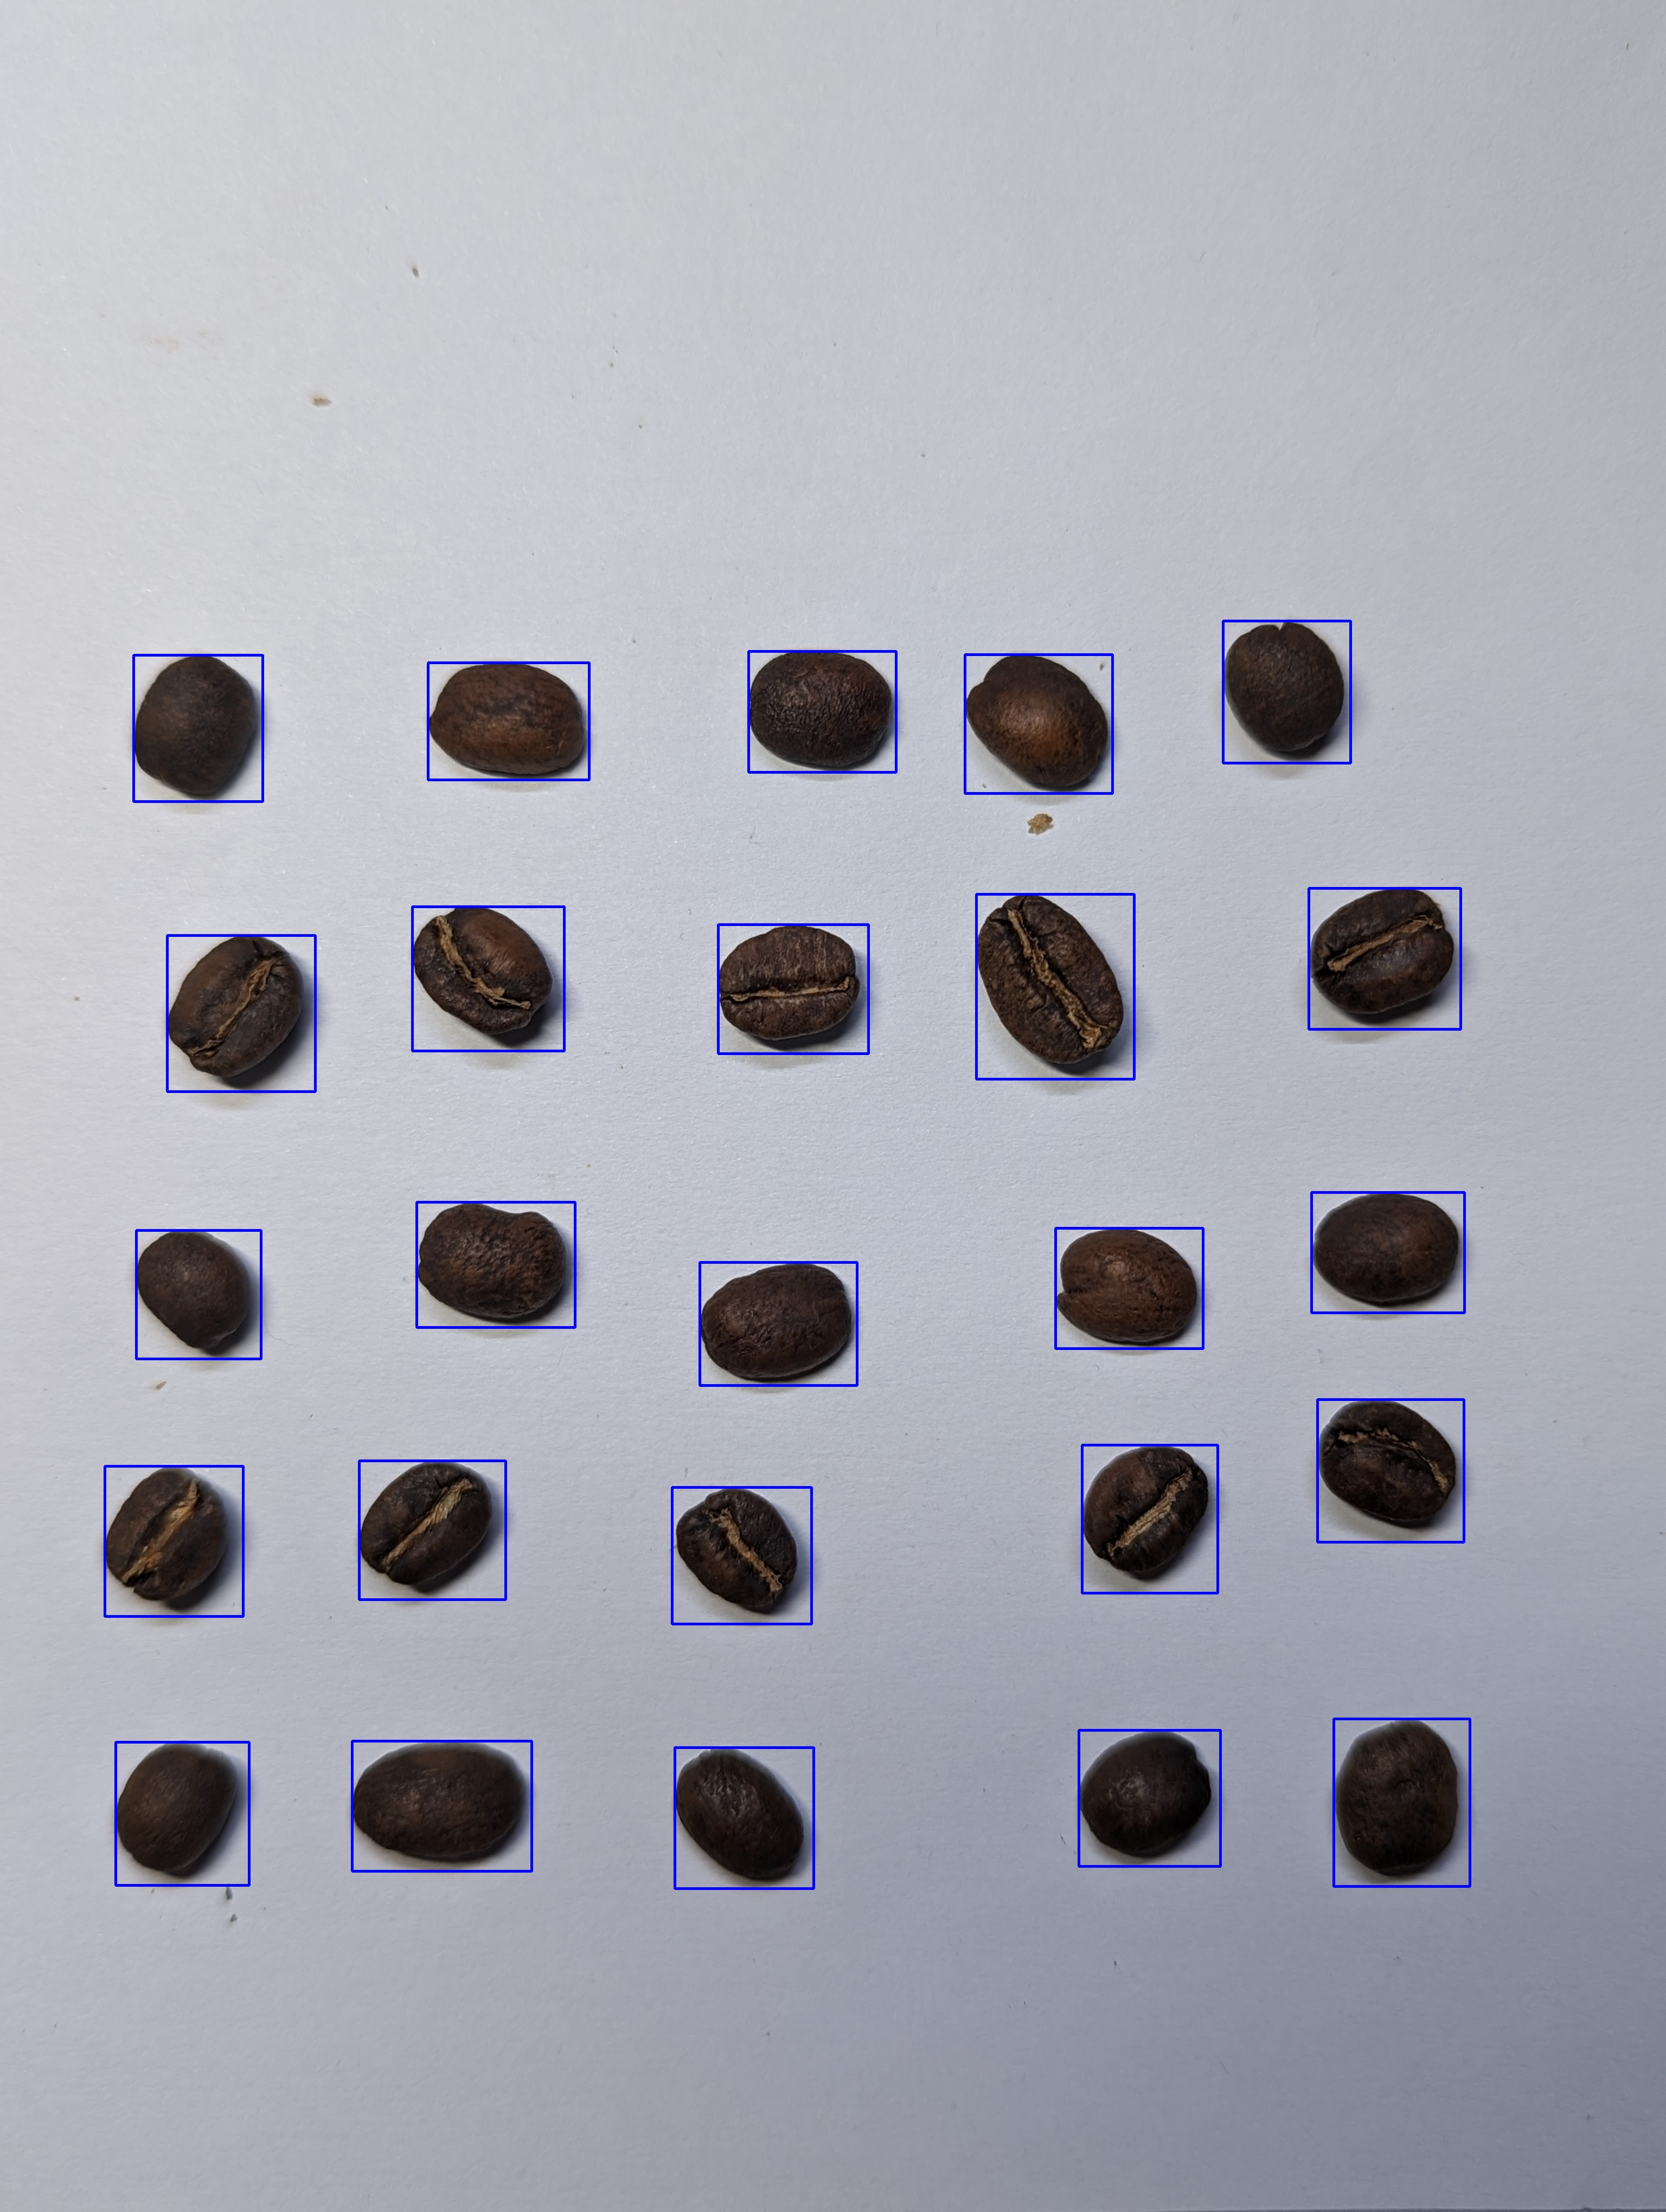
\includegraphics[height=4cm, keepaspectratio]{methodology/bean-batch-contours}};
	\node[below=of gray] (thresh)
		{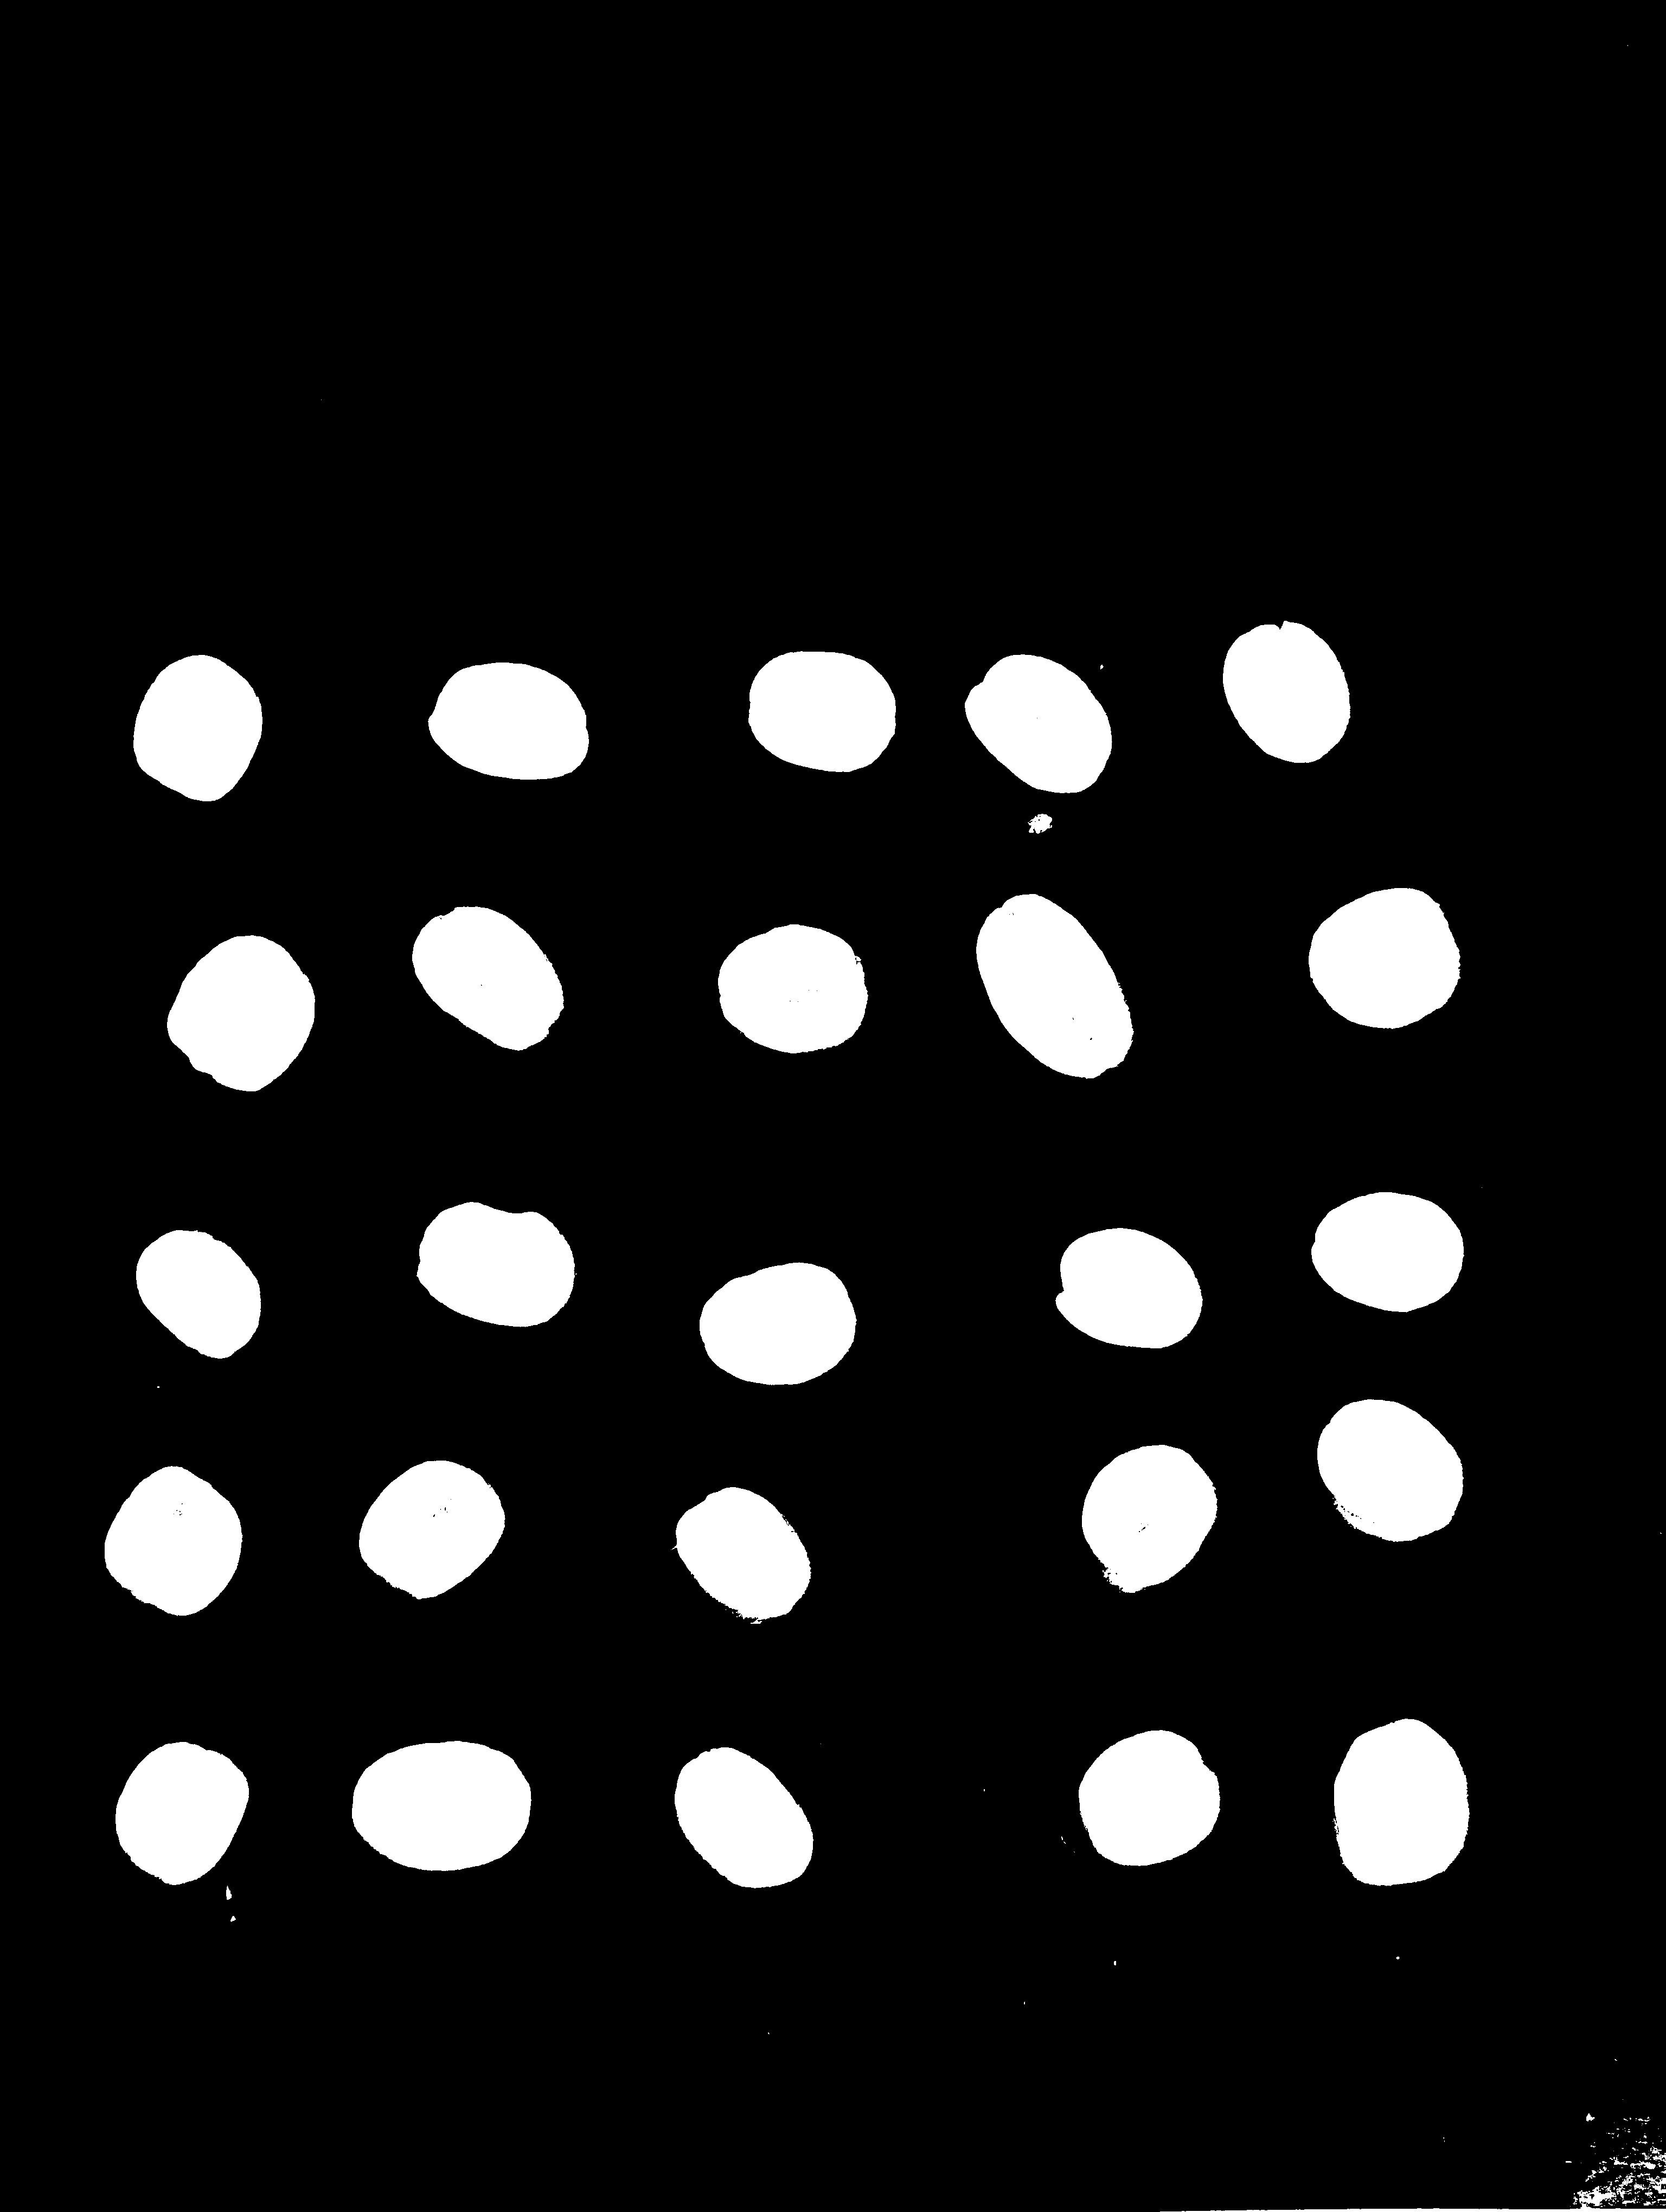
\includegraphics[height=4cm, keepaspectratio]{methodology/bean-batch-thresh}};

	\draw[->,thick] (raw) -- (gray);
	\draw[->,thick] (gray) -- (thresh);
	\draw[->,thick] (thresh) -- (contours);
\end{tikzpicture}
	\caption{Image processing pipeline}
	\label{fig:imgProcessing}
\end{figure}

Overall, the data processing pipeline yielded a dataset containing the individual images in a nested directory, with
a CSV annotations file in the top-level directory.
This structure allowed the images to be easily accessed by a machine learning framework, allowing progress towards the
aims of the project.


\section{Approaches to model development}
\label{sec:approaches-to-model-development}
The following section outlines the approaches taken in implementing a suite of image classifiers for bean defects.
The classifiers were implemented in Python, and, where applicable, were trained on an M3 Apple Silicon system with 36GB
of memory.
\subsection{Unsupervised learning}
\label{subsec:knn-classifier}

\subsection{Compact CNN classifier}
\label{subsec:deep-learning}

\subsection{Application of transfer learning to large models}
\label{subsec:transfer-learning}

\section{Model development results}
\label{sec:model-development-results}